\documentclass[mathserif]{beamer}

\usepackage{nips15}

%-----------------------------------------------------------------------
\usepackage{pdfpages}
\usepackage{array}
\usepackage[skins,breakable]{tcolorbox}
\usepackage{minibox}
\usepackage{mathtools}

\newcommand{\qcite}[1]{{\scriptsize\color{col2}[#1]}}
\newcommand{\qbox}[1]{%
\begin{tcolorbox}[enhanced jigsaw,size=tight,hbox,boxsep=4pt,boxrule=1pt,coltext=black,colframe=col1light,colback=col1,opacityback=0.7,opacityframe=1]
\strut #1
\end{tcolorbox}%
}
\newcommand{\qtheorem}[1]{%
\begin{tcolorbox}[enhanced jigsaw,size=tight,boxsep=7pt,boxrule=1pt,coltext=textcolor,colframe=col2,colback=col1,opacityback=0,opacityframe=1]
\begin{minipage}{\textwidth}
{\color{col2}\strut Theorem}\\[0.7em]
#1
\end{minipage}
\end{tcolorbox}%
}
%-----------------------------------------------------------------------

\title[Sampling from Probabilistic Submodular Models]
{Sampling from Probabilistic Submodular Models}

\author[Alkis Gotovos]{
\vspace{1in}
\normalsize
\parbox{1in}{Alkis Gotovos\\{\footnotesize ETH Zurich}}\and
\parbox{1in}{Hamed Hassani\\{\footnotesize ETH Zurich}}\and
\parbox{1in}{Andreas Krause\\{\footnotesize ETH Zurich}}
}

\begin{document}

\setbeamertemplate{background canvas}{}
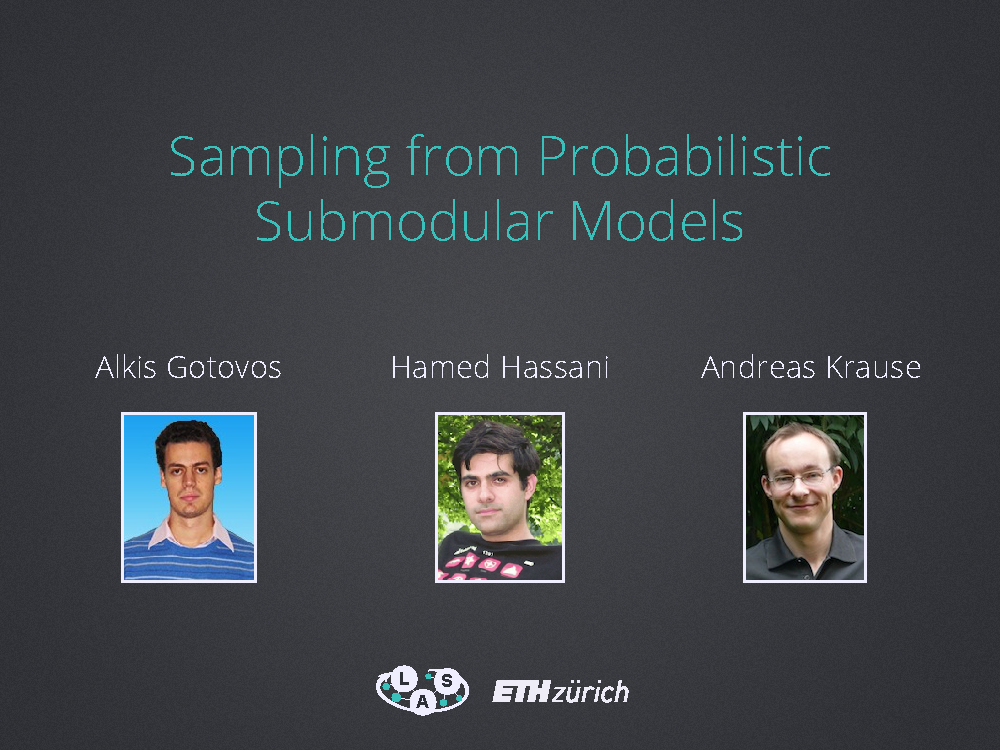
\includepdf[pages={1}]{title.pdf}
\setbeamertemplate{background canvas}{
\includegraphics[width=\paperwidth]{figures/bg.png}}

\begin{frame}{Markov Chain Monte Carlo}
\begin{tabular}{*{2}{@{}l}}
\begin{minipage}{0.45\textwidth}
\begin{itemize}
\item State space $\Omega$
\end{itemize}
\end{minipage} & \color{col1}subset lattice on $V$\\[1em]
\begin{minipage}{0.45\textwidth}
\begin{itemize}
\item Transition matrix $P$
\end{itemize}
\end{minipage} & \color{col1}Gibbs sampler
\end{tabular}

\vspace{3em}
Define Markov chain $\left(X_t\right)_t$ that moves according to $P$

\vspace{2em}
\begin{tabular}{*{2}{@{}l}}
\begin{minipage}{0.45\textwidth}
\begin{itemize}
\item Stationary distribution $\pi$
\end{itemize}
\end{minipage} & \color{col1}PSM distribution
\end{tabular}
\end{frame}

\begin{frame}{Markov Chain Monte Carlo}
\vspace{0.5em}
\centering
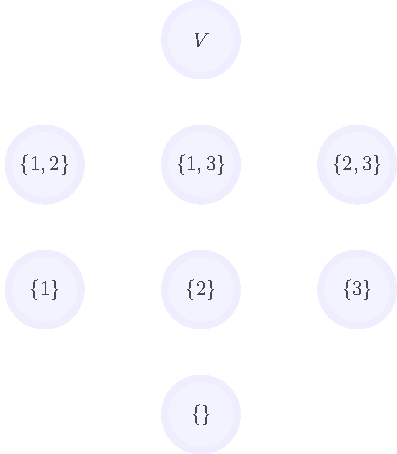
\includegraphics[height=3in]{figures/lattice_nodes_only.pdf}
\end{frame}

\begin{frame}{Markov Chain Monte Carlo}
\vspace{0.5em}
\centering
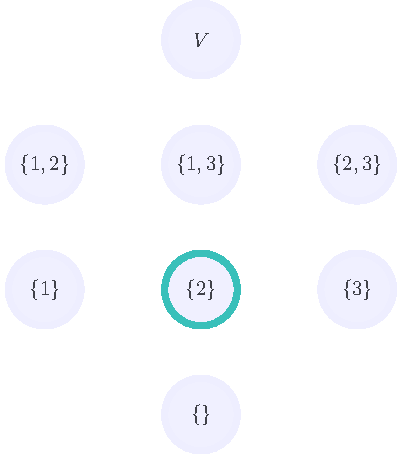
\includegraphics[height=3in]{figures/lattice_example_node.pdf}
\end{frame}

\begin{frame}{Markov Chain Monte Carlo}
\vspace{0.5em}
\centering
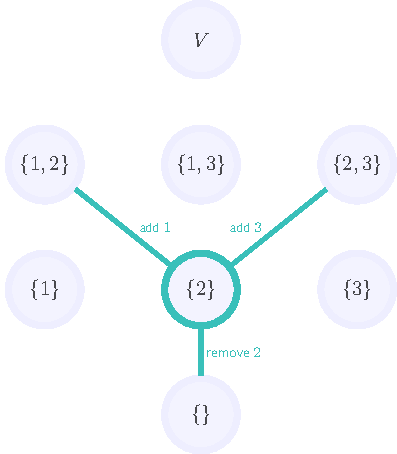
\includegraphics[height=3in]{figures/lattice_example_edges.pdf}
\end{frame}

\begin{frame}{Markov Chain Monte Carlo}
\vspace{0.5em}
\centering
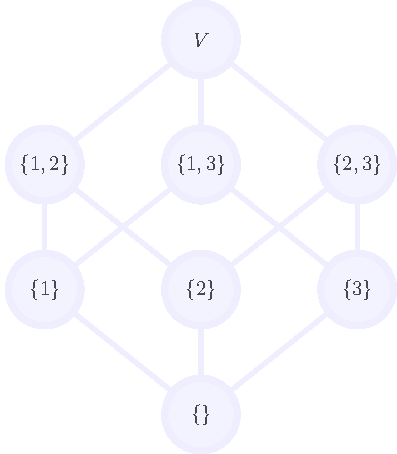
\includegraphics[height=3in]{figures/lattice_full.pdf}
\end{frame}

\begin{frame}{Markov Chain Monte Carlo}
\vspace{0.5em}
\centering
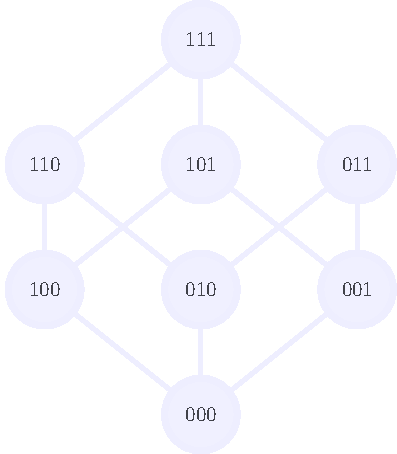
\includegraphics[height=3in]{figures/lattice_full_binary.pdf}
\end{frame}

\begin{frame}{Gibbs Sampler for PSMs}
\vspace{1em}
Start at $X_0$

\vspace{1.1em}
For $t = 1, 2, \ldots$
\vspace{1.1em}
\begin{itemize}
\item Select random $v \in V$
\vspace{1.1em}
\item $\Delta \leftarrow F(X_t \cup \{v\}) - F(X_t \setminus \{v\})$
\vspace{1.1em}
\item $p_{\textrm{add}} \leftarrow e^{\beta \Delta} / \left(1 + e^{\beta \Delta}\right)$
\vspace{1.1em}
\item Flip biased coin

\vspace{-1em}
\begin{minipage}{0.5\textwidth}\vspace{2em}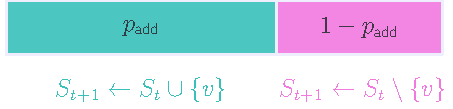
\includegraphics[width=2.7in]{figures/gibbs.pdf}\end{minipage}
\end{itemize}
\end{frame}

\begin{frame}{Mixing time}
\vspace{1em}
Total variation distance
\only<1>{
\begin{align*}
d(t) = d_{\mathrm{tv}}\left(\mathbb{P}_{X_t}, \pi\right)
\end{align*}}
\only<2>{
\begin{align*}
d(t) = {\color{col1}\max \{}d_{\mathrm{tv}}\left(\mathbb{P}_{X_t}, \pi\right) {\color{col1}\mid X_0 \in \Omega\}}
\end{align*}
}
\uncover<3->{
\begin{align*}
d(t) = \max \{d_{\mathrm{tv}}\left(\mathbb{P}_{X_t}, \pi\right) \mid X_0 \in \Omega\}
\end{align*}
}

\uncover<3->{
\vspace{1em}
Under mild assumptions (ergodicity),
\begin{align*}
d(t) \xrightarrow{\ t\,\rightarrow\,\infty\ } 0
\end{align*}
}

\uncover<4->{
\qbox{How long does it take to get ``close enough" to $\pi$?}
}

\uncover<5->{
\vspace{1em}
Mixing time
\begin{align*}
t_{\textrm{mix}}(\epsilon) = \min \left\{t \mid d(t) \leq \epsilon \right\}
\end{align*}
}
\end{frame}

\begin{frame}{Mixing time}
Mixing times for general PSMs are exponential in $|V|$

\vspace{1em}
Exponential even for pairwise models \qcite{Jerrum and Sinclair, '93}

\vspace{4em}
\qbox{\minibox{We establish sufficient conditions for sub-exponential mixing\\of the Gibbs sampler on PSMs.}}
\end{frame}

\begin{frame}{Polynomial-time Mixing}
\vspace{0.5em}
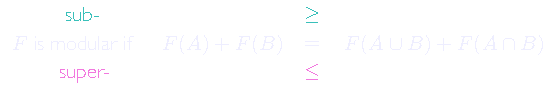
\includegraphics[width=3.9in,trim=5 0 0 0,clip]{figures/ineq_mod.pdf}

\vspace{4em}
``Distance" from modularity
\begin{align*}
\zeta_F \coloneqq \max_{A, B \subseteq V} \big|F(A) + F(B) - F(A \cup B) - F(A \cap B)\big|
\end{align*}
\end{frame}

\begin{frame}{Polynomial-time Mixing}
\qtheorem{
For any set function $F$, the mixing time of the Gibbs sampler is bounded by
\vspace{-1em}
\begin{align*}
t_{\textrm{mix}} \leq 2n^2 \exp(2\beta\zeta_F)\log\left(\displaystyle\frac{1}{\epsilon p_{\textrm{min}}}\right).
\end{align*}
}
\end{frame}

\begin{frame}{Polynomial-time Mixing}
\qtheorem{
For any set function $F$, the mixing time of the Gibbs sampler is bounded by
\vspace{-1em}
\begin{align*}
t_{\textrm{mix}} \leq 2n^2 \exp(2\beta\zeta_F)\log\left(\displaystyle\frac{1}{\epsilon p_{\textrm{min}}}\right).
\end{align*}

\vspace{0.5em}
If $F$ is submodular or supermodular the bound is improved to
\begin{align*}
t_{\textrm{mix}} \leq 2n^2 \exp(\beta\zeta_f)\log\left(\displaystyle\frac{1}{\epsilon p_{\textrm{min}}}\right).
\end{align*}
}
\end{frame}

\begin{frame}{Polynomial-time Mixing}
\qtheorem{
For any set function $F$, the mixing time of the Gibbs sampler is bounded by
\vspace{-1em}
\begin{align*}
t_{\textrm{mix}} \leq 2n^2 \exp({\color{col2}2}\beta\zeta_{\color{col2}F})\log\left(\displaystyle\frac{1}{\epsilon p_{\textrm{min}}}\right).
\end{align*}

\vspace{0.5em}
If $F$ is submodular or supermodular the bound is improved to
\begin{align*}
t_{\textrm{mix}} \leq 2n^2 \exp(\beta\zeta_{\color{col2}f})\log\left(\displaystyle\frac{1}{\epsilon p_{\textrm{min}}}\right).
\end{align*}
}
\end{frame}

\end{document}
